% Copyright (C) 2014 Miquel Sabaté Solà <mikisabate@gmail.com>
%
% This program is free software: you can redistribute it and/or modify
% it under the terms of the GNU General Public License as published by
% the Free Software Foundation, either version 3 of the License, or
% (at your option) any later version.
%
% This program is distributed in the hope that it will be useful,
% but WITHOUT ANY WARRANTY; without even the implied warranty of
% MERCHANTABILITY or FITNESS FOR A PARTICULAR PURPOSE.  See the
% GNU General Public License for more details.
%
% You should have received a copy of the GNU General Public License
% along with this program.  If not, see <http://www.gnu.org/licenses/>.

\documentclass[12pt]{beamer}
\usetheme{beamr}
\usepackage[utf8]{inputenc}

%%
% Info about the document to be generated.

\pdfinfo
{
  /Title       (Lecture)
  /Creator     (Miquel Sabaté Solà)
  /Author      (Miquel Sabaté Solà)
}

\title{Stream processing with Storm}
\author{Miquel Sabaté Solà}
\date{June 27, 2014}

\begin{document}

\frame{\titlepage}

%%
% Content starts here

\begin{frame}
\vfill
  \frametitle{The problem}
  \begin{itemize}
    \item Cities start to embrace technology.
    \vfill
    \item There's a lot of realtime data to be processed.
    \vfill
    \item Different sets of data.
    \vfill
    \item iCity
    \vfill
  \end{itemize}
\vfill
\end{frame}

\begin{frame}
\vfill
  \frametitle{The idea}
  \begin{itemize}
    \item Build a platform that:
    \vfill
    \begin{itemize}
      \item Fetches and processes data in realtime.
      \vfill
      \item Provides an easy way to extend it.
      \vfill
      \item Wraps the iCity API, instead of replacing it.
    \end{itemize}
  \end{itemize}
\vfill
\end{frame}

\begin{frame}
\vfill
  \frametitle{Goals}
  \begin{quotation}
    The {\bf goal} of this project is to build a base platform that is able to
generate rich information about a set of cities in real time.
  \end{quotation}

  \begin{itemize}
    \item Design a base platform.
    \vfill
    \item Design a couple of useful services.
    \vfill
    \item An ideal cluster.
  \end{itemize}
\vfill
\end{frame}

\begin{frame}
\vfill
  \frametitle{Technologies}
  \begin{itemize}
    \item Linux.
    \vfill
    \item Java \& Scala.
    \vfill
    \item Storm.
    \vfill
    \item Cassandra.
    \vfill
    \item Go.
    \vfill
  \end{itemize}
\vfill
\end{frame}

\begin{frame}
\vfill
  \frametitle{An overview}
  \begin{center}
    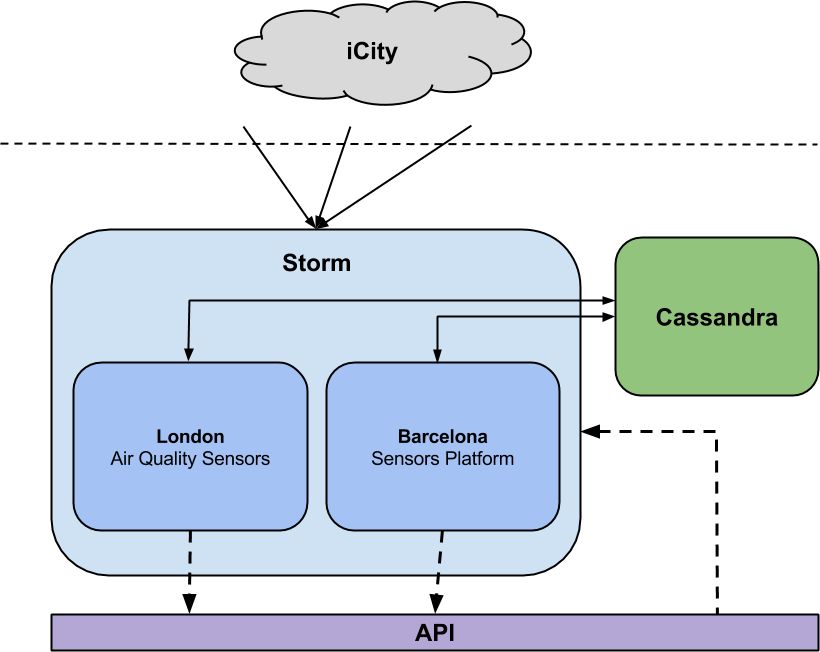
\includegraphics[scale=0.4]{images/arch.png}
  \end{center}
\vfill
\end{frame}

\begin{frame}
\vfill
  \frametitle{The Storm application}
  \begin{itemize}
    \item The com.mssola.snacker.core package.
    \vfill
    \item The AQS service as a traditional API.
    \vfill
    \item The BSP as a streaming API.
    \vfill
  \end{itemize}
\vfill
\end{frame}

\begin{frame}
\vfill
  \frametitle{API}
  \begin{center}
    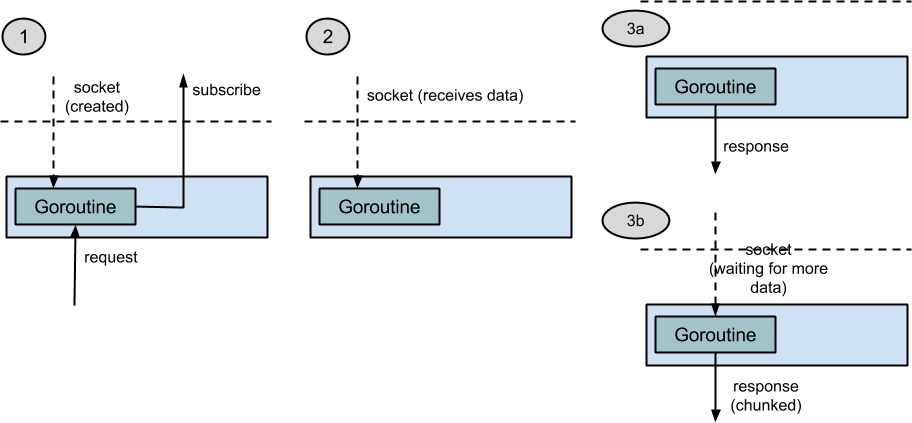
\includegraphics[scale=0.45]{images/api.png}
  \end{center}
\vfill
\end{frame}

\begin{frame}
\vfill
  \frametitle{Demo 1}
  \begin{center}
    \huge Demo 1
  \end{center}
\vfill
\end{frame}


\begin{frame}
\vfill
  \frametitle{Demo 2}
  \begin{center}
    \huge Demo 2
  \end{center}
\vfill
\end{frame}

\begin{frame}
\vfill
  \frametitle{Requirements \& limits}
  \begin{center}
    \begin{itemize}
      \item Normal execution.
      \item Benchmark
      \item Conclusions:
    \end{itemize}
    \vbox{}
    \begin{tabular}{ | c | c | c | }
      \hline
      Component & Minimum & Recommended \\ \hline
      Memory & 900 MB & 2 GB \\
      CPU & No minimum & multi-core \\
      Disk storage & 2 MB & keep it simple \\ \hline
    \end{tabular}
  \end{center}
\vfill
\end{frame}

\begin{frame}
\vfill
  \frametitle{Social \& environmental impact}
  \begin{itemize}
    \item The burden of maintaining a cluster:
    \vfill
    \begin{itemize}
      \item Power supply.
      \vfill
      \item Maintaining a cooling system.
      \vfill
      \item Building the cluster.
      \vfill
    \end{itemize}
    \vfill
    \item Social impact:
    \vfill
    \begin{itemize}
      \item Local economy.
      \vfill
      \item How citizens interact.
      \vfill
    \end{itemize}

  \end{itemize}
\vfill
\end{frame}

\begin{frame}
\vfill
  \frametitle{Conclusions}
  \begin{itemize}
    \item Meeting the expectations.
    \vfill
    \item The future.
    \vfill
  \end{itemize}
\vfill
\end{frame}

\begin{frame}
\vfill
  \frametitle{Questions}
  \begin{center}
    \vfill
    
\includegraphics[scale=0.15]{images/questions.png}
    \vfill
  \end{center}
\vfill
\end{frame}

\end{document}
